\documentclass[12pt]{article}
\usepackage{graphicx}
\usepackage{amsmath}
\usepackage{verbatim}
\begin{document}

\begin{titlepage}
\title{
Report on Analytic Solution for Annular Ducts}


\author{ Jeff Severino
 \\
University of Toledo \\
Toledo, OH  43606 \\
email: jseveri@rockets.utoledo.edu  }

\maketitle

\end{titlepage}

\section{Introduction - Current Research Direction}
The \verb|FORTRAN 77| codes that compute the duct mode solution for annular ducts are
presented.  A testing routine written in FORTRAN 90 calls the FORTRAN 77 subroutines, 
the main one being \verb|rmode.f|. The weigting factors, $A$, and $B$ as well as
the roots that satisfy the transcendental equation containing the determinant of 
the derivative of the bessel functions of the first and second kind.  By importing
$A$, $B$, and the nondimensional roots into \verb|Python|, the modeshape result
from FORTRAN was validated. For a complete validation, $A$, $B$, and the 
nondimensional roots should be computed in \verb|Python|, however this is not 
necessary since there is no restriction to using \verb|F77|.


  
\section{Research Performed}
\subsection{Numerical Computation of Annular Duct Modes}
\subsubsection{Theoretical Background}

The analytic radial mode shape is of the form,

\begin{equation}
    R_m(k_{r,mn} r) =  A J_m (k_{r,mn} r) + B Y_m (k_{r,nmn} r)
\end{equation}
The key to the numerical procedure is the following ``transcendental'' equation,
\begin{equation}
    \begin{vmatrix}
        J'_m(k_{r,mn} r_H) &Y'_m(k_{r,mn} r_H) \\
        J'_m(k_{r,mn} r_T) &Y'_m(k_{r,mn} r_T) 
    \end{vmatrix}   
    = 0
\end{equation}
 The non-dimensional roots $k_{r,mn} r_T$ are found using initial guess and then incrementing from there

 \begin{equation}
     k_{r,mn} = 
    \begin{cases}
        m & \text{if } n = 1\\
        k_{r,m(n-1)} r_T + \pi,              & \text{if }  n > 1.
    \end{cases}
 \end{equation}

 The estimate is refined by incrementing the value of $k_{r,mn}$ by $\pi/10$ until
 the determinant above changes sign. The step size is then halved and also changes 
 sign. This iterative process continues until the absolute value of the determinant 
 is reduced to a preassigned error tolerance. The non dimensional versions
 of these equations are used in the FORTRAN 77 Code, \verb|anrt.f|, which calls 
 \verb|anfu.f|.

 Once $k_{r,mn}$ has been computed, the weighting factors $A$ and $B$ are assigned to 
 one of the following two sets of values ( \verb|eigen.f|)
 \begin{equation*}
     \begin{cases}
         A = 1 \\ 
         B = - \frac{J'_m(k_{r,mn} r_H )}{Y'_m(k_{r,mn} r_H )}
     \end{cases}
     \text{or,}
     \begin{cases}
         A =- \frac{Y'_m(k_{r,mn} r_H )}{J'_m(k_{r,mn} r_H )}  \\
         B = 1
     \end{cases}
 \end{equation*}
Of these two values, which ever has the smaller $A^2 + B^2$ is chosen.

The desired normalization,

\begin{equation}
    \int_{r_T}^{r_H} R_m^2(k_{r,mn} r) r dr = \frac{1}{2}\left( r_T^2-r_H^2 \right)
    \label{eqn:desirednormalization}
\end{equation}

is obtained by computing the value on the left-hand side of 
Equation (\ref{eqn:desirednormalization}) using the expression,

\begin{equation}
    \int_{r_H}^{r_T} R_m^2(k_{r,mn} r) r dr = 
    \frac{1}{2}\left( r^2 - \frac{m^2}{k_{r,mn}^2} \right)R_m^2 (k_{r,mn} r)\Big|_{r = r_H}^{r_T} \equiv C
\end{equation}

The constants $A$ and $B$ are divided by,

\begin{equation}
    \sqrt{\frac{2C}{\left( r_T^2 - r_H^2 \right)}}
    \label{eqn:normalizationconst}
\end{equation}
to give the normalization needed in Equation (\ref{eqn:desirednormalization}) 

The non-dimensionalization in this code uses the following,
\[ X_{mn} = k_{r,mn} r_T\]
\[ x = r/r_T\]
\[ \sigma = r_H/r_T\]

The non-dimensional equivalent expressions are 

\begin{equation}
    \int_{\sigma}^{1} R_m^2(X_{mn} x) x dr = \frac{1}{2}\left( 1 - \sigma^2 \right)
    \label{eqn:desirednormalization_nondimensional}
\end{equation}

\begin{equation}
    \int_{\sigma}^{1} R_m^2(X_{mn} x) x dr = 
    \frac{1}{2}\left( x^2 - \frac{m^2}{X_{mn}^2} \right)R_m^2 (X_{mn} x)\Big|_{x = \sigma}^{1}
\end{equation}
and the constant that A and B are divided by becomes 

\begin{equation}
    \sqrt{\frac{
\left( 1 - \frac{m^2}{X_{mn}^2} \right)R_m^2 (X_{mn} )  -
\left( \sigma^2 - \frac{m^2}{X_{mn}^2} \right)R_m^2 (X_{mn} \sigma)
}{\left( 1 - \sigma^2 \right)}}
    \label{eqn:normalizationconst_nondimension}
\end{equation}

The current code is in the Appendix, which produces the following:

\begin{figure}
    \centering
    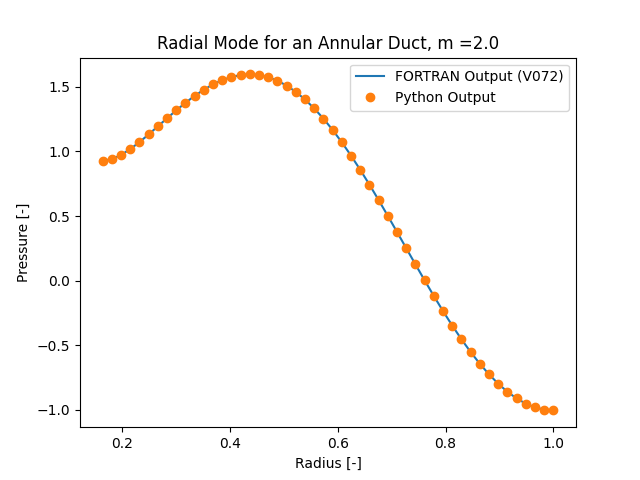
\includegraphics{../figures/Figure1.png}
    \caption{initial result}
    \label{fig:dd}
\end{figure}

\begin{figure}
    \centering
    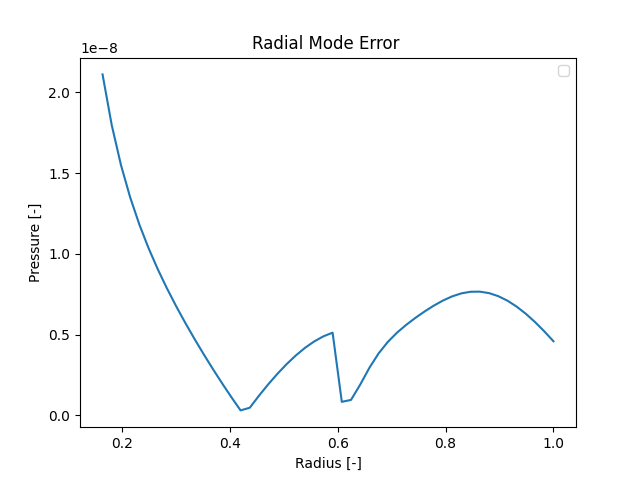
\includegraphics{../figures/Figure1error.png}
    \caption{initial result}
    \label{fig:d}
\end{figure}

\begin{figure}
    \centering
    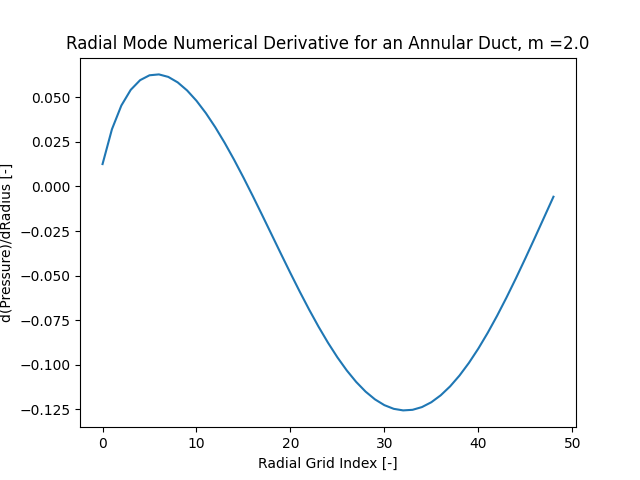
\includegraphics{../figures/Figure1deriv.png}
    \caption{initial result}
    \label{fig:d}
\end{figure}

Figure \ref{fig:dd} shows the radial mode 3. The two lines are used as a sanity 
check to ensure that 1) The bessel function routines work in F77 2) and so that 
my understanding of the F77 routines is intact. 


\section{Issues and Concerns}
The only issue I have now is the current state of SWIRL. The modes that are 
computed in SWIRL have very poor filtering and sorting methods for the eigenvalue 
problem. For this reason, the relevant radial modes and their corresponding wavenumber 
were sorted in post. I have to do the annular modes in post too if I want the 
answer as soon as possible. Once a case study is done there, perhaps I can add the 
sorting functionality that I worked on in Python to Fortran.



\section{Planned Research} 
\subsubsection{Validation - Annular Duct Modes}
Set test case parameters and compare results to SWIRL.
\subsubsection{Validation - Cylindrical Duct Modes}

I believe I have a potential technical memorandum with the boundary condition issues 
in the cylindrical case. I'd like to ``make the case'' for this by reporting the 
rates of convergence for the first 5 modes at 5-6 grids. The notes from my discussion
with Envia help me make this case! I did a preliminary literature review, 
\cite{meyer1996aeroacoustic}
\section{Appendix}

\subsection{Code Documention}

\begin{itemize}
    \item \verb|eigen.f|, 
        \subitem Computes the weighting factors, $A$ and $B$ for the radial mode
        shpe
    \item \verb|besj.f|, 
        \subitem Computes the bessel functions of the first kind and their derivatives
        of positive or zero order, n, and zero or positive argument x 
    \item \verb|besy.f|, and 
        \subitem Computes the bessel function of the second kind and their 
        derivatives of positive or zero order, n, and zero or positive argument x 
    \item \verb|rmode.f|. 
        \subitem Calculate radial mode shape psi for the (m,n) radial mode of an annular duct 
\end{itemize}

Currently a subdirectory within the \verb|v070_nasalib| directory has a testing 
code to obtain the annular duct modes. 
\begin{verbatim}

! BesselFunctionCode
! Author - Jeff Severino
! Date - 11/17/22
!
! Description -
! This code tests various subroutines in the v070nasalib needed to produce 
! a radial mode shape for annular ducts
!
PROGRAM BesselFunctionCode
      USE, INTRINSIC :: ISO_FORTRAN_ENV  
      IMPLICIT NONE

      INTEGER, PARAMETER :: &
          rDef = REAL64, &
          numberOfGridPoints = 50

      LOGICAL :: &
          debug_flag = .FALSE.

      CHARACTER(LEN = 50) :: &
          filename

      INTEGER :: &
          UNIT                  ,&
          azimuthal_mode_number ,&
          radial_mode_number    ,&
          i
      
      
      REAL(KIND=rDef) :: & 
          r_min, &
          r_max, &
          dr,  &
          weighting_coefficient_A, &
          weighting_coefficient_B, &
          hubTipRatio,&
          convergence_criteria ,& 
          mode_shape

      REAL(KIND=rDef), DIMENSION(:), ALLOCATABLE :: &
          radial_grid

      REAL(KIND=rDef),DIMENSION(2) :: &
          rmode_bessel_function_errors

      REAL(KIND=rDef),DIMENSION(4) :: &
          eigen_bessel_function_errors , &
          anfu_bessel_function_errors 

      REAL(KIND=rDef) :: &
          anrt_convergence_flag 
      
      REAL(KIND=rDef) :: &
          non_dimensional_roots


      ALLOCATE(radial_grid(numberOfGridPoints))


      r_min = 0.20_rDef 
      r_max = 1.0_rDef      
      azimuthal_mode_number = 2 
      radial_mode_number = 3
      convergence_criteria = 1.0E-12_rDef
      hubTipRatio = r_min/r_max 

      dr    = (r_max-r_min)/REAL(numberOfGridPoints-1, rDef)

      DO i =1,numberOfGridPoints

      radial_grid(i)  = (r_min+REAL(i-1, rDef)*dr)!radial grid 
      
      ENDDO
      
      CALL ANRT(&
          azimuthal_mode_number,&
          radial_mode_number,&
          hubTipRatio,&
          convergence_criteria,&
          non_dimensional_roots,&
          anfu_bessel_function_errors,&
          anrt_convergence_flag)

      ! checking ANRT result

      IF (anrt_convergence_flag .gt. 0.0_rDef) THEN
          WRITE(0,*) 'ERROR: ANRT DID NOT CONVERGE ',anrt_convergence_flag
      ELSE
      ENDIF

      IF (debug_flag.eqv..TRUE.) THEN
          ! WRITE(0,*) 'k_mn r_max' ,non_dimensional_roots
      ELSE
      ENDIF
      
      ! Obtaining A and B coefficients for radial mode shape

      CALL EIGEN(&
          azimuthal_mode_number, &
          hubTipRatio          , &
          non_dimensional_roots, &
          weighting_coefficient_A                  , &
          weighting_coefficient_B                  , &
          eigen_bessel_function_errors)

      IF (debug_flag.eqv..TRUE.) THEN
          WRITE(0,*) 'A ' , weighting_coefficient_A
          WRITE(0,*) 'B ' , weighting_coefficient_B
          WRITE(0,*) 'k_mn r_max ' , non_dimensional_roots
          WRITE(0,*) 'k_mn ' , non_dimensional_roots/r_max
      ELSE
      ENDIF

      filename = 'radial_mode_data.dat'
      OPEN(NEWUNIT=UNIT,FILE=TRIM(ADJUSTL(filename))) 

      WRITE(UNIT,*) &
          'radius ', &
          'pressure '
       
      DO i = 1,numberOfGridPoints

      CALL RMODE(&
      azimuthal_mode_number,&
      non_dimensional_roots*radial_grid(i)/r_max,&
      weighting_coefficient_A,&
      weighting_coefficient_B,&
      mode_shape,&
      rmode_bessel_function_errors)
  
      WRITE(UNIT,*) &
          radial_grid(i)/r_max,&
          mode_shape 

      ENDDO

      CLOSE(UNIT)

      IF (debug_flag) THEN
          OPEN(NEWUNIT=UNIT,FILE='radial_mode_parameters.dat')
          WRITE(UNIT,*) &
              'azimuthal_mode_number ', &
              'radial_mode_number ', &
              'weighting_factor_A ', &
              'weighting_factor_B ', &
              'non_dimensional_roots ' 
          WRITE(UNIT,*) &
              azimuthal_mode_number, &
              radial_mode_number , &
              weighting_coefficient_A, &
              weighting_coefficient_B, &
              non_dimensional_roots 
          CLOSE(UNIT)
      ENDIF
END PROGRAM
! Notes:
! Pros of f90 for V072:
!   better management of inputs and outputs
!       - explicit interfaces
\end{verbatim}

plotting code, \verb|plotResult.py|
\begin{verbatim}

#!/usr/bin/env python3
import matplotlib
import matplotlib.pyplot as plt
import pandas as pd
import pprint 
import scipy as scip
import numpy as np

debug_flag = False

filename = 'radial_mode_data.dat'
parameter_filename = 'radial_mode_parameters.dat'
data = \
        pd.read_csv(filename, delim_whitespace = True)

if debug_flag:
   pprint.pprint(data)

parameters = \
        pd.read_csv(parameter_filename, delim_whitespace = True)
if debug_flag:
    pprint.pprint(parameters)

AMN =float(parameters['weighting_factor_A'])
BMN =float(parameters['weighting_factor_B'])
k_rmn = float(parameters['non_dimensional_roots'])
m_order = float(parameters['azimuthal_mode_number'])

pressure_python = \
        (AMN)*scip.special.jv(m_order,k_rmn*(data['radius'])) + \
        (BMN)*scip.special.yv(m_order,k_rmn*(data['radius']))

fig, axs = plt.subplots()

axs.plot(
        data['radius'],
        data['pressure'],
        label = 'FORTRAN Output (V072)')

axs.plot(data['radius'],pressure_python,'o',label = 'Python Output')

plt.title('Radial Mode for an Annular Duct, m =' + str(m_order))
plt.xlabel('Radius [-]')
plt.ylabel('Pressure [-]')
plt.legend()

plt.savefig('docs/figures/Figure1.png')

fig, axs = plt.subplots()
axs.plot(np.diff(data['pressure']))

plt.title('Radial Mode Numerical Derivative for an Annular Duct, m =' + str(m_order))
plt.xlabel('Radial Grid Index [-]')
plt.ylabel('d(Pressure)/dRadius [-]')

plt.show()



\end{verbatim}

 \end{document}
